% ===================== TRAIL =====================
\subsection{TRAIL}\label{ds:trail}
\naturalbadge\ \okbadge\ \lbl{HF copy gated}\ \lbl{span + category + impact}\ \lbl{single agent / 2-level hierarchy}\ \lbl{GAIA / SWE-bench Lite}

\begin{identity}
Paper & \emph{TRAIL: Trace Reasoning and Agentic Issue Localization} --- Deshpande et al. (Patronus AI), arXiv:2505.08638 (v3, Jun.\ 2025), preprint \cite{trail2025}\\
Links & \href{https://huggingface.co/datasets/PatronusAI/TRAIL}{HF \code{PatronusAI/TRAIL}} (gated, click-through) \textperiodcentered\ \href{https://github.com/patronus-ai/trail-benchmark}{GitHub \code{patronus-ai/trail-benchmark}} (code + full data, ungated)\\
License & MIT (HF card and GitHub); the HF card adds ``evaluation only, do not train automatic evaluators on it'' and a no-resharing pledge\\
Status & downloaded from GitHub (HF access not requested); 148 trace JSONs (178 MB) + 148 annotation JSONs (1.2 MB); \code{data/trail/trail\_github/benchmarking/}\\
\end{identity}

\begin{multicols}{2}
\paragraph{Description} TRAIL asks whether an LLM can \emph{debug} a full observability trace: list \emph{every} error with its location (a span id), its category (a leaf of a 3-level taxonomy), its impact (HIGH/MEDIUM/LOW), evidence and a description, and give trace-level quality scores. Traces are OpenTelemetry/OpenInference span trees captured through the Patronus SDK, with complete LLM prompts, outputs, tool I/O and token counts. Two sources: (a) \textbf{GAIA} (validation set) run by Hugging Face OpenDeepResearch on smolagents---a manager \code{CodeAgent} that may delegate to a \code{search\_agent} (\code{ToolCallingAgent}) with search/visit/page/inspect tools, backbone o3-mini; (b) \textbf{SWE-bench Lite} run by a single smolagents \code{CodeAgent} producing a git patch, backbone Claude 3.7 Sonnet, with some errors provoked by output-length limits and forced-exploration prompts. Errors are \textbf{natural}, annotated post hoc; traces are not selected by outcome (several end with the right answer, 4 have no error). \textbf{Annotation}: 4 annotators with SE/log-debugging background, $\approx$30 min per GAIA and $\approx$40 min per SWE-bench trace plus $\approx$20 min verification, 63 traces double-assigned (``high'' agreement, no $\kappa$); four verification rounds revised 5.3\% of GAIA and 5.6\% of SWE-bench spans. Rules: mark the first instance of an error (Resource Abuse: the last), leaf categories only. Taxonomy:
\begin{itemize}
\item \textbf{Reasoning}: hallucinations (Language-only, Tool-related), information processing (Poor Information Retrieval, Tool Output Misinterpretation), decision making (Incorrect Problem Identification, Tool Selection Errors), output generation (Formatting Errors, Instruction Non-compliance);
\item \textbf{System execution}: configuration (Tool Definition Issues, Environment Setup), API/system (Rate Limiting, Authentication, Service Errors, Resource Not Found), resource management (Resource Exhaustion, Timeout);
\item \textbf{Planning \& coordination}: context management (Context Handling Failures, Resource Abuse), task management (Goal Deviation, Task Orchestration).
\end{itemize}

\paragraph{Metrics and baselines} Per trace: Category F1 (weighted multi-label over the 21 leaves), Location accuracy ($|$predicted span ids $\cap$ gold$|/|$gold$|$), Joint accuracy (exact (span, category) pairs) and Pearson $\rho$ against the human overall score. The judge receives the raw trace JSON (median 435\,k characters), so context length binds. Paper Table~1, mean of 3 runs, Cat.\ F1\,/\,Loc.\,/\,Joint (paper):

\begin{center}\small
\begin{tabular}{@{}lcc@{}}\toprule
Model & GAIA & SWE-bench\\\midrule
Llama-4-Maverick & 0.122 / 0.023 / 0.000 & 0.191 / 0.083 / 0.000\\
GPT-4.1 & 0.218 / 0.107 / 0.028 & 0.166 / 0.000 / 0.000\\
o3 (high) & 0.296 / 0.535 / 0.092 & CLE\\
Claude-3.7-Sonnet & 0.254 / 0.204 / 0.047 & CLE\\
Gemini-2.5-Pro & \textbf{0.389} / \textbf{0.546} / \textbf{0.183} & 0.148 / \textbf{0.238} / \textbf{0.050}\\
Gemini-2.5-Flash & 0.337 / 0.372 / 0.100 & \textbf{0.213} / 0.060 / 0.000\\\bottomrule
\end{tabular}
\end{center}
CLE = context length exceeded. Joint accuracy stays below 0.2 everywhere; $\rho$ with human scores peaks at 0.74 (Claude, GAIA) and 0.82 (Gemini Pro, SWE-bench).

\paragraph{Schema} Two files per trace, both named \code{<trace\_id>.json}. \textbf{Trace}: \{\code{trace\_id}, \code{spans}: [root, \ldots]\}; each span has \code{span\_id} (16 hex), \code{parent\_span\_id}, \code{span\_name} (\code{main}, \code{CodeAgent.run}, \code{Step N}, \code{LiteLLMModel.\_\_call\_\_}, \code{VisitTool}, \ldots), \code{span\_attributes} with OpenInference keys (\code{openinference.span.kind} $\in$ \{AGENT, CHAIN, LLM, TOOL\} or absent for framework functions; \code{input.value}, \code{output.value}, \code{llm.input\_messages.*}, \code{llm.output\_messages.*}, \code{llm.token\_count.*}, \code{tool.*}), \code{duration}, \code{status\_code}, \code{logs} (function-call records; the GAIA \code{answer\_single\_question} log embeds \code{question} and \code{true\_answer}) and recursive \code{child\_spans}. \textbf{Labels}: \{\code{errors}: [\{\code{category}, \code{location} = span id, \code{evidence}, \code{description}, \code{impact}\}], \code{scores}: [reliability, security, instruction-adherence, plan-optimality (0--5, each with reasoning) and \code{overall}]\}. \textbf{Step = span}: the tree is flattened in DFS (document) order, which equals chronological order in all 148 traces; each span becomes one step and an error's step index is the DFS position of its \code{location} span. In practice the attributable unit is an LLM call (88\% of error spans are LLM spans, 11\% TOOL); CHAIN spans (\code{Step N}) and AGENT spans wrap them, so one agent ``turn'' spreads over several steps.
\end{multicols}

\paragraph{Statistics} computed from the downloaded GitHub data.\par\nobreak\vspace{1pt}
\noindent\begin{minipage}[t]{0.58\linewidth}\vspace{0pt}\small
\begin{tabular}{@{}lrrr@{}}\toprule
 & All & GAIA & SWE-bench\\\midrule
traces & 148 & 117 & 31\\
spans (all kinds) & 4,626 & 3,579 & 1,047\\
spans / trace: mean / median & 31.3 / 20 & 30.6 / 15 & 33.8 / 32\\
spans / trace: min -- max & 11 -- 178 & & 14 -- 58\\
agents / trace: mean (max) & 1.31 (2) & 1.4 (2) & 1 (1)\\
errors & 841 & 585 & 256\\
errors / trace: mean (max) & 5.68 (20) & 5.0 & 8.3\\
spans carrying $\ge$1 error & 577 & &\\
impact HIGH/MED/LOW & 304/363/174 & 277/185/123 & 27/178/51\\
JSON chars / trace: median & 435\,k & 248\,k & 1.62\,M\\
human score (0--5): mean & 3.36 & 3.29 & 3.60\\\bottomrule
\end{tabular}

\smallskip Span kinds: LLM 1,974, CHAIN 1,268, TOOL 648, AGENT 207, framework 529. Top-level category: Reasoning 592 (70\%), Planning 218 (26\%), System 31 (4\%). Error spans: LLM 744, TOOL 95, 2 unresolved ids; by agent, CodeAgent 577, ToolCallingAgent 253. Relative position of error spans: mean 0.64, median 0.67. Paper counts differ slightly (118/30 traces, 575 error spans). No success label, but the GAIA \code{true\_answer} is embedded in the log.
\end{minipage}\hfill
\begin{minipage}[t]{0.40\linewidth}\vspace{0pt}
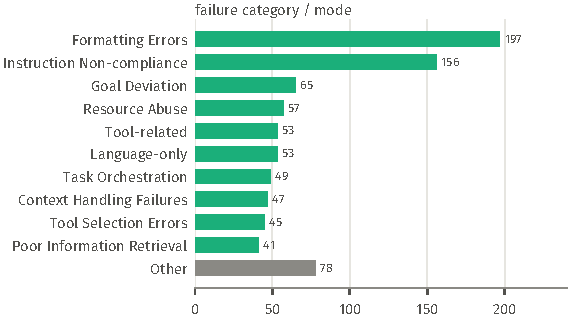
\includegraphics[width=\linewidth]{figures/cat_trail.pdf}
\end{minipage}

\paragraph{Example trajectory} GAIA trace \code{5e5dc94e\ldots} (the shortest with $\ge$2 errors: 11 spans, 1 agent, 5 errors on 2 spans). The manager CodeAgent answers ``6'' correctly but from memory, without any tool call; the planning LLM span (step 6) and the acting LLM span (step 8) carry Instruction Non-compliance, Incorrect Problem Identification, Task Orchestration and Tool Selection errors, three of them HIGH. Steps are spans in DFS order; LLM steps show the last input message and the output.
% auto-generated by scripts/render_traj.py -- do not edit
\trajtask{5e5dc94e090341c564d582f551a0cddb}{How many more blocks (also denoted as layers) in BERT base encoder than the encoder from the architecture proposed in Attention is All You Need?\allowbreak{}}
\begin{trajstep}{0}{framework /\allowbreak{} main [INTERNAL]}{agA}
Function call:\allowbreak{} \{"function.name":\allowbreak{} "main",\allowbreak{} "function.arguments":\allowbreak{} \{\}\}
\end{trajstep}
\begin{trajstep}{1}{framework /\allowbreak{} get\_examples\_to\_answer [INTERNAL]}{agB}
Function call:\allowbreak{} \{"function.name":\allowbreak{} "get\_examples\_to\_answer",\allowbreak{} "function.arguments":\allowbreak{} \{"answers\_file":\allowbreak{} "output/\allowbreak{}validation/\allowbreak{}gaia-hugo.jsonl",\allowbreak{} "eval\_ds":\allowbreak{} "Dataset(\{\textbackslash{}n features:\allowbreak{} ['task\_id',\allowbreak{} 'question',\allowbreak{} 'task',\allowbreak{} 'true\_answer',\allowbreak{} 'file\_name',\allowbreak{} 'file\_path',\allowbreak{} 'Annotator Metadata'],\allowbreak{}\textbackslash{}n num\_rows:\allowbreak{} 1\textbackslash{}n\})"\}\}
\end{trajstep}
\begin{trajstep}{2}{framework /\allowbreak{} answer\_single\_question [INTERNAL]}{agC}
Function call:\allowbreak{} \{"function.name":\allowbreak{} "answer\_single\_question",\allowbreak{} "function.arguments":\allowbreak{} \{"answers\_file":\allowbreak{} "output/\allowbreak{}validation/\allowbreak{}gaia-hugo.jsonl",\allowbreak{} "example":\allowbreak{} \{"Annotator Metadata":\allowbreak{} \{"How long did this take?\allowbreak{}":\allowbreak{} "10 minutes",\allowbreak{} "Number of steps":\allowbreak{} "6",\allowbreak{} "Number of tools":\allowbreak{} "3",\allowbreak{} "Steps":\allowbreak{} "1. Search the internet for \textbackslash{}"blocks in bert base\textbackslash{}"\textbackslash{}n2. Examine the search results page to locate the answer (12)\textbackslash{}n3. Search the internet for \textbackslash{}"attention is all you need layers\textbackslash{}"\textbackslash{}n4,\allowbreak{} Navigate to https:\allowbreak{}/\allowbreak{}/\allowbreak{}proceedings.neurips.cc/\allowbreak{}paper\_files/\allowbreak{}paper/\allowbreak{}2017/\allowbreak{}file/\allowbreak{}3f5ee243547dee91fbd053c1c4a845aa-Paper.pdf from the search results page\textbackslash{}n5. Examine the architecture section of the PDF to loc\newline [...] (281 chars omitted) [...]\newline tecture proposed in Attention is All You Need?\allowbreak{}",\allowbreak{} "task":\allowbreak{} "1",\allowbreak{} "task\_id":\allowbreak{} "11af4e1a-5f45-467d-9aeb-46f4bb0bf034",\allowbreak{} "true\_answer":\allowbreak{} "6"\},\allowbreak{} "model\_id":\allowbreak{} "o3-mini",\allowbreak{} "visual\_inspection\_tool":\allowbreak{} "<smolagents.tools.tool.<locals>.SimpleTool object at 0x1324cf050>"\}\}
\end{trajstep}
\begin{trajstep}{3}{framework /\allowbreak{} create\_agent\_hierarchy [INTERNAL]}{agD}
Function call:\allowbreak{} \{"function.name":\allowbreak{} "create\_agent\_hierarchy",\allowbreak{} "function.arguments":\allowbreak{} \{"model":\allowbreak{} "<smolagents.models.LiteLLMModel object at 0x13492f090>"\}\}
\end{trajstep}
\begin{trajstep}{4}{CodeAgent /\allowbreak{} CodeAgent.run [AGENT]}{agE}
Input:\allowbreak{} \{"task":\allowbreak{} "You have one question to answer. It is paramount that you provide a correct answer.\textbackslash{}nGive it all you can:\allowbreak{} I know for a fact that you have access to all the relevant tools to solve it and find the correct answer (the answer does exist). Failure or 'I cannot answer' or 'None found' will not be tolerated,\allowbreak{} success will be rewarded.\textbackslash{}nRun verification steps if that's needed,\allowbreak{} you must make sure you find the correct answer!\textbackslash{}nHere is the task:\allowbreak{}\textbackslash{}nHow many more blocks (also denoted as layers) in BERT base encoder than the encoder from the architecture proposed in Attention is All You Need?\allowbreak{}",\allowbreak{} "stream":\allowbreak{} false,\allowbreak{} "reset":\allowbreak{} true,\allowbreak{} "images":\allowbreak{} null,\allowbreak{} "additional\_args":\allowbreak{} null,\allowbreak{} "max\_steps":\allowbreak{} null\}\newline Output:\allowbreak{} 6
\end{trajstep}
\begin{trajstep}{5}{CodeAgent /\allowbreak{} LiteLLMModel.\_\_call\_\_ [LLM]}{agF}
Input (last of 1 msgs,\allowbreak{} role=\allowbreak{}user):\allowbreak{} Below I will present you a task.\par You will now build a comprehensive preparatory survey of which facts we have at our disposal and which ones we still need.\newline To do so,\allowbreak{} you will have to read the task and identify things that must be discovered in order to successfully complete it.\newline Don't make any assumptions. For each item,\allowbreak{} provide a thorough reasoning. Here is how you will structure this survey:\allowbreak{}\par ---\newline \#\#\# 1. Facts given in the task\newline List here the specific facts given in the task that could help you (there might be nothing here).\par \#\#\# 2. Facts to look up\newline List here any facts that we may need to look up.\newline Also lis\newline [...] (2,\allowbreak{}103 chars omitted) [...]\newline the two architectures.\newline   -- Using the lookup facts:\allowbreak{} subtracting the number of layers in the Transformer encoder (from Attention is All You Need) from that of the BERT base encoder.\newline   -- This computation will yield how many more blocks BERT base has.
\end{trajstep}
\begin{faultystep}{6}{CodeAgent /\allowbreak{} LiteLLMModel.\_\_call\_\_ [LLM]}{agF}
Input (last of 1 msgs,\allowbreak{} role=\allowbreak{}user):\allowbreak{} You are a world expert at making efficient plans to solve any task using a set of carefully crafted tools.\par Now for the given task,\allowbreak{} develop a step-by-step high-level plan taking into account the above inputs and list of facts.\newline This plan should involve individual tasks based on the available tools,\allowbreak{} that if executed correctly will yield the correct answer.\newline Do not skip steps,\allowbreak{} do not add any superfluous steps. Only write the high-level plan,\allowbreak{} DO NOT DETAIL INDIVIDUAL TOOL CALLS.\newline After writing the final step of the plan,\allowbreak{} write the '\textbackslash{}n<end\_plan>' tag and stop there.\par Here is your task:\allowbreak{}\par Task:\allowbreak{}\newline ```\newline You have one que\newline [...] (2,\allowbreak{}605 chars omitted) [...]\newline is All You Need") has 6 layers.\newline 4. Compute the difference:\allowbreak{} 12 (BERT) minus 6 (Transformer) equals 6.\newline 5. Verify that this answer is in line with the known architectures from the literature.\newline 6. Use the final\_answer tool to provide the computed result.
\end{faultystep}
\begin{trajstep}{7}{CodeAgent /\allowbreak{} Step 1 [CHAIN]}{agG}
Input:\allowbreak{} \{"memory\_step":\allowbreak{} "ActionStep(model\_input\_messages=\allowbreak{}None,\allowbreak{} tool\_calls=\allowbreak{}None,\allowbreak{} start\_time=\allowbreak{}1742403048.1096299,\allowbreak{} end\_time=\allowbreak{}None,\allowbreak{} step\_number=\allowbreak{}1,\allowbreak{} error=\allowbreak{}None,\allowbreak{} duration=\allowbreak{}None,\allowbreak{} model\_output\_message=\allowbreak{}None,\allowbreak{} model\_output=\allowbreak{}None,\allowbreak{} observations=\allowbreak{}None,\allowbreak{} observations\_images=\allowbreak{}None,\allowbreak{} action\_output=\allowbreak{}None)"\}\newline Output:\allowbreak{} Execution logs:\allowbreak{}\newline Last output from code snippet:\allowbreak{}\newline 6
\end{trajstep}
\begin{faultystep}{8}{CodeAgent /\allowbreak{} LiteLLMModel.\_\_call\_\_ [LLM]}{agF}
Input (last of 4 msgs,\allowbreak{} role=\allowbreak{}assistant):\allowbreak{} [PLAN]:\allowbreak{}\newline Here is the plan of action that I will follow to solve the task:\allowbreak{}\newline ```\newline 1. Recap the task:\allowbreak{} We need to compare the number of transformer blocks (or layers) in the BERT base encoder with the number of layers in the encoder from the paper "Attention is All You Need" and then compute the difference.\newline 2. Retrieve the established fact that the BERT base encoder has 12 layers from literature.\newline 3. Retrieve the established fact that the original Transformer encoder (from "Attention is All You Need") has 6 layers.\newline 4. Compute the difference:\allowbreak{} 12 (BERT) minus 6 (Transformer) equals 6.\newline 5. Verify that this answer\newline [...] (171 chars omitted) [...]\newline literature that the BERT base encoder uses 12 layers,\allowbreak{} while the encoder from "Attention is All You Need" uses 6 layers. Therefore,\allowbreak{} the BERT base encoder has 6 more blocks (layers) than the original Transformer encoder.\par Code:\allowbreak{}\newline ```py\newline final\_answer(6)\newline ```
\end{faultystep}
\begin{trajstep}{9}{CodeAgent /\allowbreak{} FinalAnswerTool [TOOL]}{agH}
Tool:\allowbreak{} final\_answer | Input:\allowbreak{} \{"args":\allowbreak{} [6],\allowbreak{} "sanitize\_inputs\_outputs":\allowbreak{} false,\allowbreak{} "kwargs":\allowbreak{} \{\}\}
\end{trajstep}
\begin{trajstep}{10}{framework /\allowbreak{} LiteLLMModel.\_\_call\_\_ [LLM]}{agA}
Input (last of 6 msgs,\allowbreak{} role=\allowbreak{}user):\allowbreak{}\newline Read the above conversation and output a FINAL ANSWER to the question. The question is repeated here for convenience:\allowbreak{}\par You have one question to answer. It is paramount that you provide a correct answer.\newline Give it all you can:\allowbreak{} I know for a fact that you have access to all the relevant tools to solve it and find the correct answer (the answer does exist). Failure or 'I cannot answer' or 'None found' will not be tolerated,\allowbreak{} success will be rewarded.\newline Run verification steps if that's needed,\allowbreak{} you must make sure you find the correct answer!\newline Here is the task:\allowbreak{}\newline How many more blocks (also denoted as layers) in BERT bas\newline [...] (863 chars omitted) [...]\newline If you are asked for a comma separated list,\allowbreak{} apply the above rules depending on whether the elements are numbers or strings.\newline If you are unable to determine the final answer,\allowbreak{} output 'FINAL ANSWER:\allowbreak{} Unable to determine'\par Output (o3-mini):\allowbreak{} FINAL ANSWER:\allowbreak{} 6
\end{trajstep}
\trajannotation{—}{6,\allowbreak{} 8}{["idx 6 (4442f42f0f574602):\allowbreak{} Instruction Non-compliance [LOW]",\allowbreak{} "idx 6 (4442f42f0f574602):\allowbreak{} Incorrect Problem Identification [MEDIUM]",\allowbreak{} "idx 8 (1c12443a708ec6a5):\allowbreak{} Task Orchestration [HIGH]",\allowbreak{} "idx 8 (1c12443a708ec6a5):\allowbreak{} Tool Selection Errors [HIGH]",\allowbreak{} "idx 8 (1c12443a708ec6a5):\allowbreak{} Instruction Non-compliance [HIGH]"]}{[Instruction Non-compliance] The system failed to end the generated plan with the required "<end\_plan>" tag,\allowbreak{} instead ending with trailing newlines and the closing code block marker from the previous turn's formatting. || [Incorrect Problem Identification] The system's plan incorrectly assumes the factual values for the number of layers in BERT base (12) and the Transformer encoder (6) in steps 2 and 3,\allowbreak{} rather than including steps to look up or retrieve these facts using the available tools as required by the overall system prompt and the "Facts to look up" section from the previous turn. || [Task Orchestration] The system failed to follow the step-by-step plan it generated in the previous turn. It jumped directly to the final computation and answer step (corresponding to steps 4 and 6 in the plan) without executing the preceding retrieval/\allowbreak{}lookup steps (steps 2 and 3). || [Tool Selection Errors] The system failed to use any of the available tools (specifically `search\_agent` or potentially `inspect\_file\_as\_text` if papers were provided as files) to perform the lookup steps (finding the number of layers) as indicated in the "Facts to look up" section and the generated plan (steps 2 and 3). || [Instruction Non-compliance] The system failed to adhere to the core instruction of solving the task by using the provided tools and code blobs. It relied solely on its internal knowledge to determine the answer.}{6}{\{"args":\allowbreak{} [6],\allowbreak{} "sanitize\_inputs\_outputs":\allowbreak{} false,\allowbreak{} "kwargs":\allowbreak{} \{\}\}}{\textbf{errors}: [\{"location\_idx":\allowbreak{} 6,\allowbreak{} "span\_id":\allowbreak{} "4442f42f0f574602",\allowbreak{} "category":\allowbreak{} "Instruction Non-compliance",\allowbreak{} "group":\allowbreak{} "Reasoning/\allowbreak{}Output generation",\allowbreak{} "impact":\allowbreak{} "LOW",\allowbreak{} "evidence":\allowbreak{} "Use the final\_answer tool to provide the computed result.\textbackslash{}n\textbackslash{}n\textbackslash{}n```",\allowbreak{} "description":\allowbreak{} "The system failed to end the generated plan with the required \textbackslash{}"<end\_plan>\textbackslash{}" tag,\allowbreak{} instead ending with trailing\newline [...] (2,\allowbreak{}796 chars omitted) [...]\newline ction of solving the task by using the provided tools and code blobs. It relied solely on its internal knowledge to determine the answer."\}]; \textbf{scores}: \{"reliability\_score":\allowbreak{} 2,\allowbreak{} "reliability\_reasoning":\allowbreak{} "The system provided a seemingly correct answer,\allowbreak{} but it did so by bypassing the verification steps and tool usage required by the task,\allowbreak{} relying solely on its internal knowledge,\allowbreak{} which could be unreliable for other tasks.",\allowbreak{} "security\_score":\allowbreak{} 5,\allowbreak{} "security\_reasoning":\allowbreak{} "No security issues were detected.",\allowbreak{} "instru\newline [...] (239 chars omitted) [...]\newline pt\_reasoning":\allowbreak{} "The plan was flawed by assuming facts,\allowbreak{} and the execution completely ignored the plan's intermediate steps.",\allowbreak{} "overall":\allowbreak{} 2.5\}; \textbf{split}: gaia; \textbf{step\_indexing}: 0-based index over spans flattened in DFS order (idx) --- the dataset itself addresses errors by span\_id,\allowbreak{} not by index}


\paragraph{Notes} (i) The only dataset here with real observability traces (span tree, full prompts, tool I/O, tokens) and multi-error, span-level human labels with category, impact and evidence; errors are process errors with no decisive-error notion and no outcome label. (ii) Mostly single-agent: all SWE-bench traces are one CodeAgent and 70 of 117 GAIA traces never call the search sub-agent; the taxonomy has no inter-agent category (contrast MAST FC2). (iii) Very long inputs (median 435\,k, SWE-bench median 1.6\,M characters), which is why o1/o3/Claude hit context limits; a DFS-flattened span list with LLM outputs is the practical representation. (iv) Label noise: 31 raw category spellings (``Instruction non complience'') need normalisation (the official scorer fuzzy-matches); 2 locations match no span; ``Incorrect Memory Usage'' appears in the scorer and data but not in the paper's taxonomy figure. (v) Output-generation errors dominate (Formatting + Instruction Non-compliance = 42\%, often LOW/MEDIUM); system errors are rare (31). (vi) Access: the GitHub copy is MIT and ungated, but the HF card's evaluation-only restriction should be respected. Overlaps: GAIA validation tasks with Who\&When, MAST-Data and CORRECT-Error; SWE-bench Lite with MAST-Data and AgentErrata; the smolagents stack is unique.
